% Historical source (removed by author request): references/_OLD_Übungsaufgaben/Übungsblatt 6 - Integralrechnung/Blatt6.tex:105
\begin{ExerciseBlock}
\ExerciseHeading{7}{Fläche zwischen Funktionen}{integral_calculus_area_between_functions}
Gegeben seien die Funktion $f(x) = 2-x^2$ (grün in Abb.) und $g(x) = x$ (blau in Abb.).
	
\begin{center}
	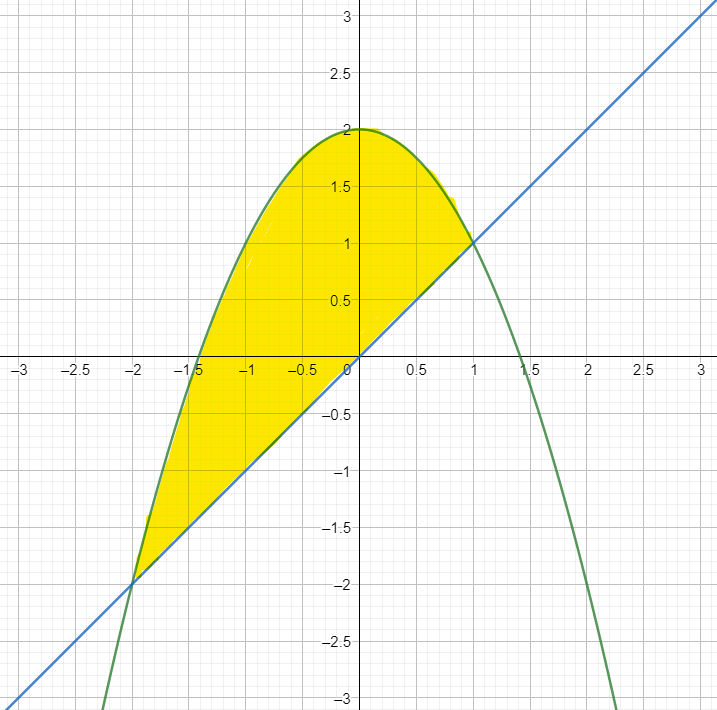
\includegraphics[width=0.6\textwidth]{content/resources/chapters/integral_calculus/images/area_between_functions.png}
\end{center}

\begin{enumerate}[label=\alph*)]
	
	\item Bestimmen Sie die beiden Schnittpunkte der Funktionen. 
	
	\item Berechnen Sie die gelb markierte Fläche, die von den beiden Funktionen eingeschlossen wird.
	
\end{enumerate}

\end{ExerciseBlock}
\UseExerciseSolution{integral_calculus_area_between_functions}
